\section{Horus Balor}

\centering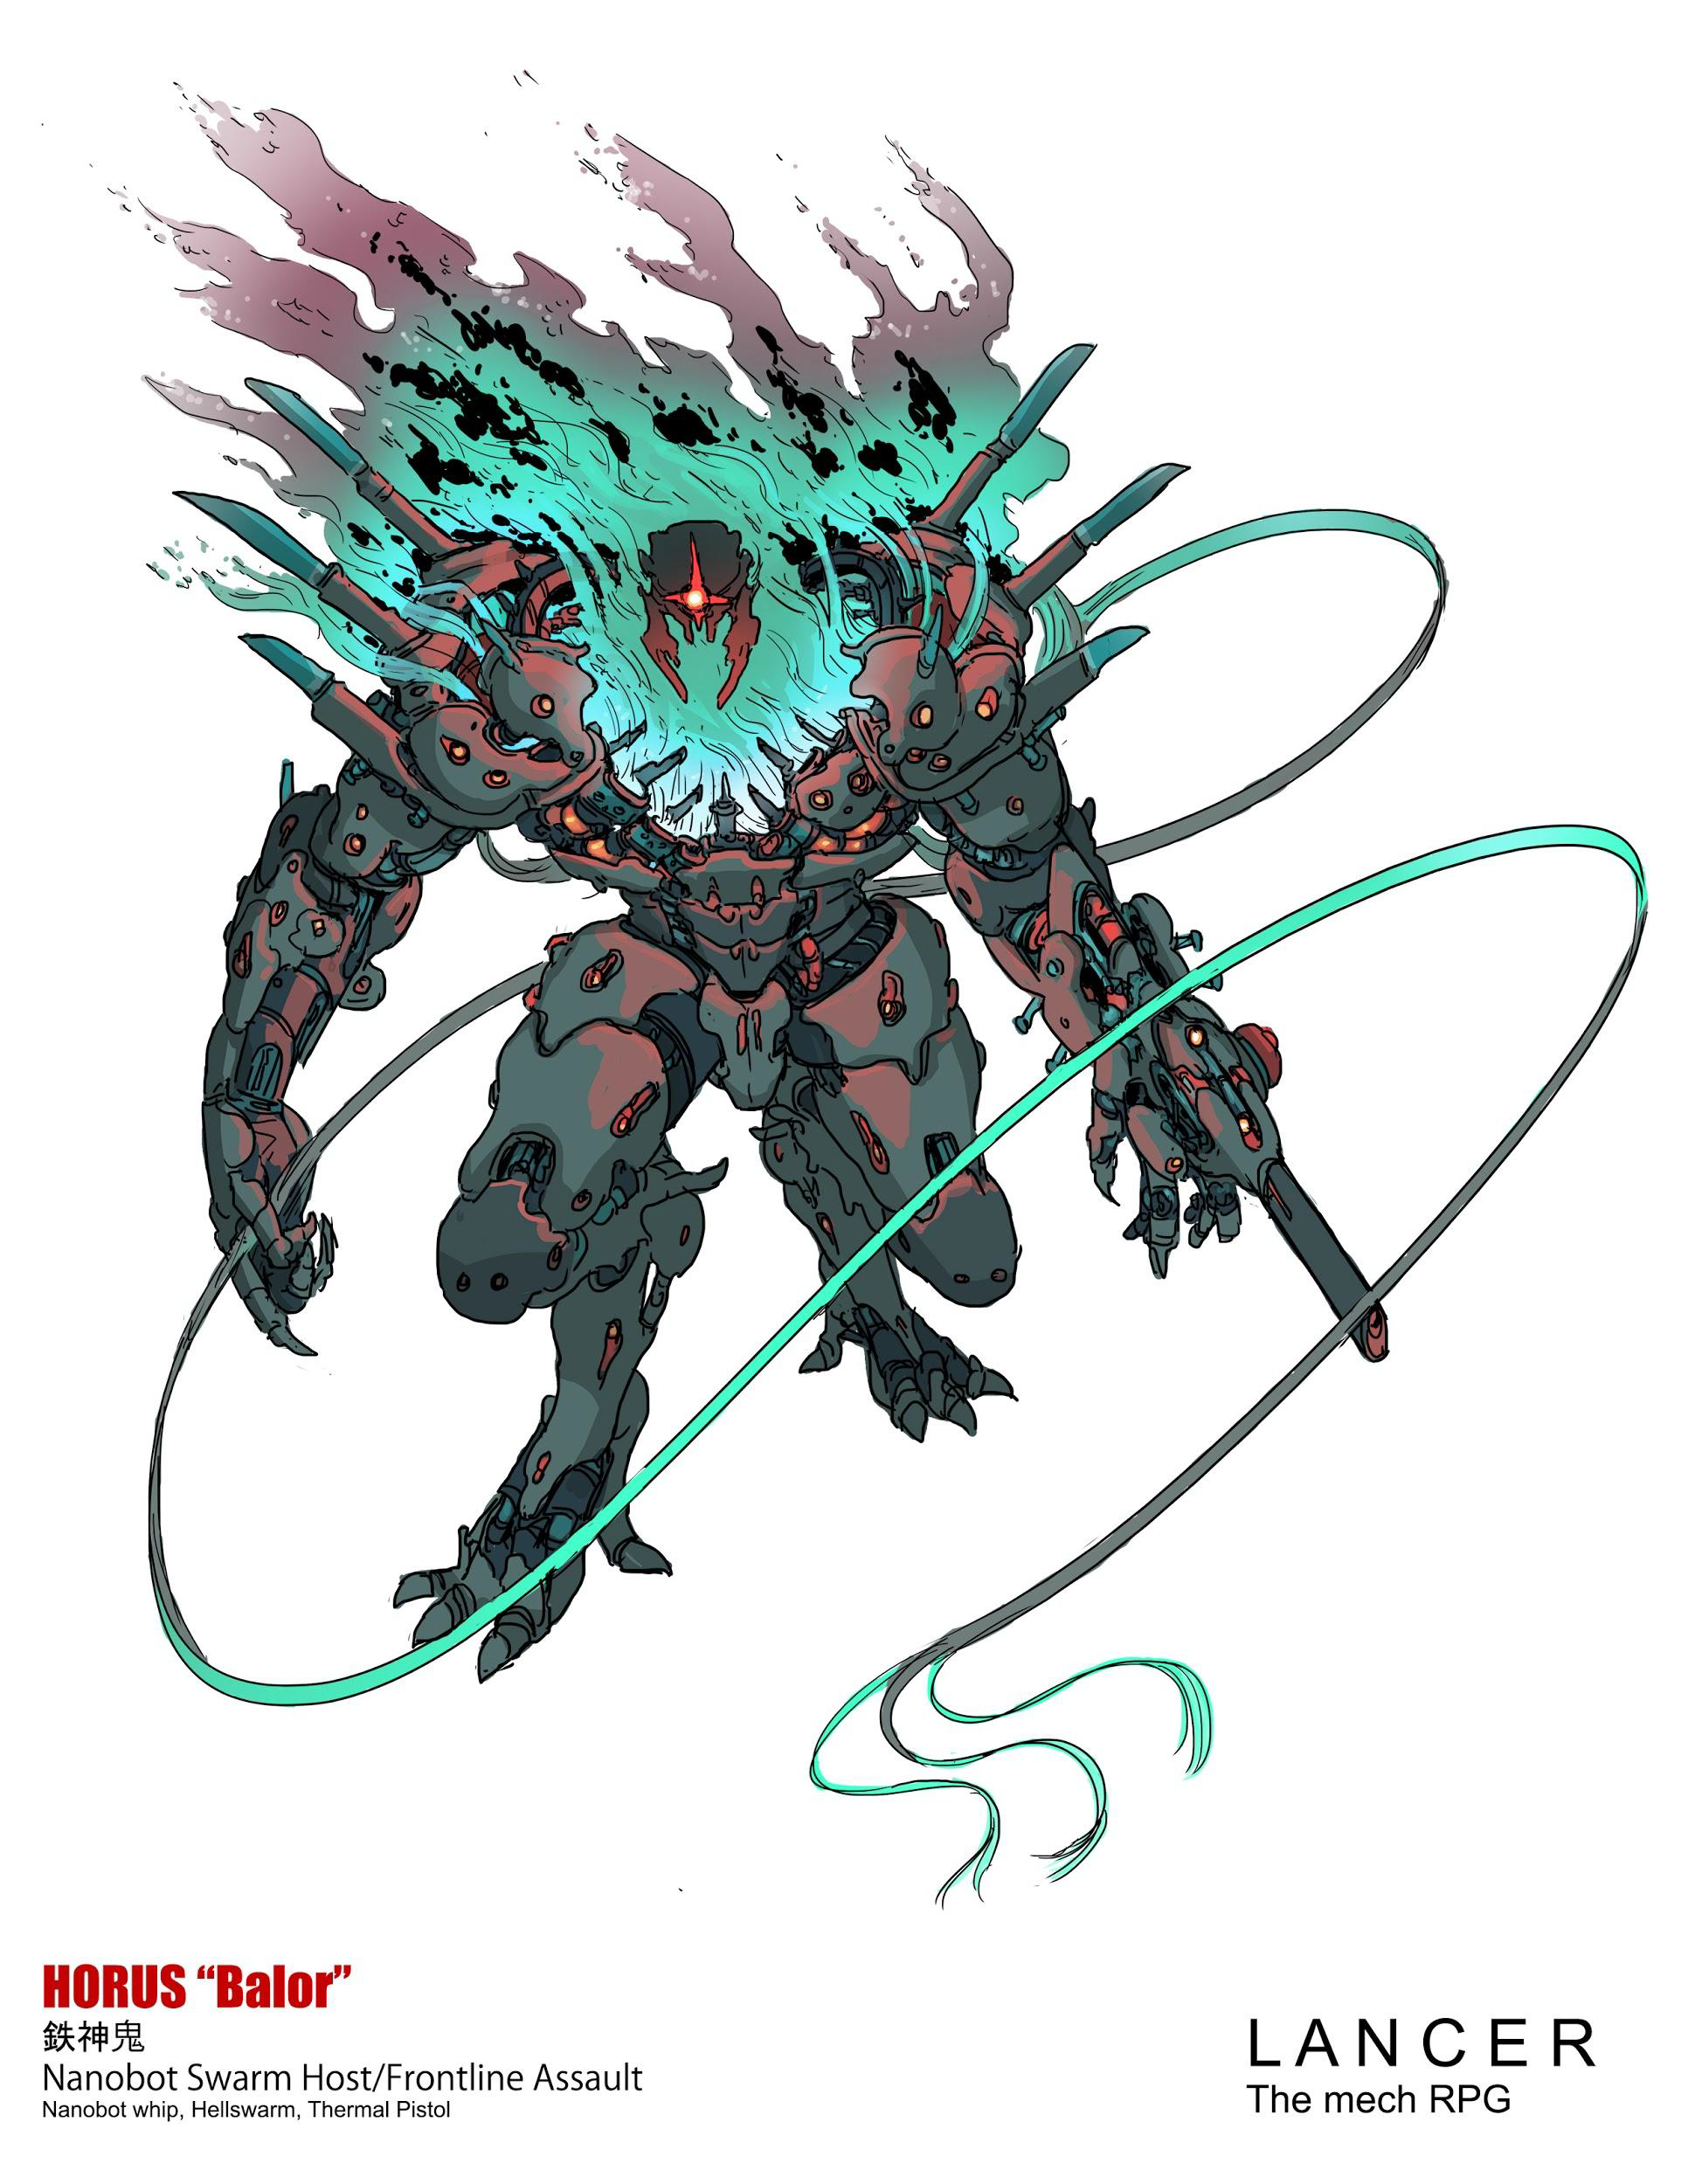
\includegraphics{Balor}

                                           HORUS BALOR

Like most all HORUS mech cores, the BALOR classification is less an indicator of a recognizable silhouette
than a general classification of intended combat role. A BALOR-rigged mech core is only stable on a larger

platform, necessitating a robust frame with multiple redundancies to prevent catastrophic system failure.
The BALOR’s neurologically synced hellswarm nanites form an undulating shroud that can pour out of its
chassis at a moment’s notice, whipping around its form defensively until weaponized.

                                                  License:
I. Scanner Swarm, Hive Drone

II. BALOR FRAME, Swarm Body, Nanocomposite materials

II. Nanobot Whip, Seeker Swarm Nexus


                                                 BALOR

 HP: 15         Evasion: 6                           Speed: 3           Heat Cap: 4       Sensors: 5

 Armor: 0       E-Defense: 10                        Size: 2            Repair Cap: 4     Tech Attack:
                                                                                          +1

                                                  TRAITS:

 Scouring Swarm: All actors of the Balor’s choice that starts their turn grappled by or adjacent to the
 Balor take 2 kinetic damage

 Regeneration: At the end of its turn in mech combat, the Balor heals 2 HP. This trait doesn’t function
 outside of combat.

                                            SYSTEM POINTS: 6

                                                 MOUNTS:

 Main Mount                                          Heavy Mount

                                               CORE system




                                                    HELLSWARM

 As one, without any command but desire, you control a cloak of millions of miniscule, quick-print
 drones: a hellswarm cloak, a living shield, a fluid-dynamic knife -- you cut and guard in one shimmering
 wave. You are Hivemaster, and your will is followed by millions.

 Active (requires 1 core power): Hive Frenzy
 Protocol
 Your swarm goes into a hyper-active mode. You can set your swarm to one of three modes, and swap
 at the start of your turn as a free action:
 Hive Shield: 1/round as a reaction, you can gain resistance to all the damage from any one attack that
 just hit you.
 Hive Repulse: While this mode is active, you have resistance to all damage from Smart, Nexus, and
  Drone weapons and systems and hostile tech actions or attacks are made at +1 difficulty against you
 Hive Scour: While this mode is active, the damage from your Scouring Swarm trait increases to 3 AP
  kinetic damage

Scanner Swarm

A HORUS-coded scanner swarm establishes a protocol for oculus-form nanites that ensures constant
circulation. The nanites ingest and process full spectrum information, relaying it back to their pilot/mother/
father for a endorphic code impulse to prompt continued scanning.

2 SP, Unique
Your Tech actions against targets in melee engagement with you gain +2 Accuracy


Hive Drone
It looks, at first, like a roiling cloud of low fog. Thick, and fizzing, like soda water spilled across concrete. It
advances with curious movement, stretching and snapping back. A confusion of snakes, sloughing forward
with speed that betrays intent.

Color flashes across the grey cloud, a kind of swarm-luminescence that, you realize, is the light created by
millions of nanites glowing with heat as they consume what they cross.

This is greywash, and it is never full.

2 SP

Drone, Quick Action


Sensor range

You can fire this drone to an empty space in sensor range as a quick action. While it’s active, it
emits a burst 2 area around it that grants light cover to any allied mech at least partially covered
by the zone (it benefits from its own cover). In addition, any hostile target that starts its turn in the
area or enters it for the first time on their turn takes 1 AP kinetic damage. You can move it to a
different space in your sensor range by repeating this action.


Swarm Body
2 SP

Quick Action





If your mech doesn’t move before the end of this turn, at the end of your turn you project a burst
1 area around your mech. Actors of your choice that move into this area for the first time on their
turns or start their turn there must pass a systems check or take 3 kinetic damage. For each turn
your mech remains immobile past the first, its damage increases by 3, up to a maximum of 9. If
your mech moves (even involuntarily), this effect immediately ends. You don’t have to take any
action to maintain it other than remaining immobile.


Nanocomposite materials

Nanite ammunition takes the principal of aggressive drone swarms and condenses it to a single round. Five
maniples of autonomous nanites are packed into a shaped CONSUME/HIVE round that shatters on positive
target impact. On impact (or airburst/ penetration detonation) the maniples are released and begin to eat

away at surrounding tissue or superstructure. They proceed until maniple burnout or total target
consumption, whichever occurs first. In flight, the maniples are able to hive-link and adjust their round’s
flight somewhat to ensure positive impact.

2 SP
Mod

Choose 1 weapon. If it’s a ranged weapon, you fire a swarm of nanobots instead of regular
ammo. If it’s a melee weapon, the entire weapon becomes made up of nanobots. The weapon
gains the Smart and Seeking properties.


Nanobot Whip

Nanobot whips are a unique protocol offered by HORUS collectivists; using swarm coding and legion
directives, HORUS collectivists created a protocol for nanites that collects them into a whip-like weapon.
This nanobot whip can retract to its base blister for stowing, and detach in melee combat to restrain nearby

enemies. The nanobot whip returns to its base unit when summoned.

Heavy Melee

2 SP

Threat 3

2d6 kinetic damage

On a Critical Hit (20+), the target must pass a systems check with 1 difficulty to scramble the
nanites or be pulled to any free adjacent space to your mech, or as far as possible while still
obeying obstructions.


Seeker Swarm nexus

The SWARM/HIVE protocol developed by HORUS collectivists is one of the more insidious weapons they
have produced. A SWARM/HIVE nanite swarm combines the systemic invasion properties of HORUS’s

BOOST/HIVE protocol with the aggressive tuning of a CONSUME/HIVE maniple. Launched from mounted
HIVE blisters, a SWARM/HIVE nanite swarm will coalesce upon an enemy, infiltrate sensitive compartments
and modules, and begin to eat away at any material they can find.

Main Nexus

Smart, Seeking





Range 5

2 kinetic damage + Burn 2
